\section{Log-linear surrogate of compute-constrained training loss}
\label{appendix:surrogate}
\subsection{Data Collection}
We collect estimates of the $K$-step (“compute-constrained”) training loss
\(
  \mathcal{L}_{\mathrm{trn}}(\theta;|m|)
\)
at a range of subset sizes $|m|$.  By default we choose nine relative fractions
$\{0.01,0.02,0.05,0.1,0.3,0.5,0.7,0.9\}$ of the full training set
(clamped to at least 50 examples on MNIST or the configured batch‐size otherwise).
For each size we train for a total compute budget $N$ (so that each inner training run sees roughly the same total number of gradient steps), and record the final training loss. We then summarize each size by its empirical~$\ell_j$.

\subsection{Surrogate model choice}
We set \(\varepsilon=10^{-10}\) and fit the transformed log‐loss
\(\log\bigl(l(|m|)+\varepsilon\bigr)\) using two options:
\begin{itemize}
  \item \textbf{Linear:}  
    \(\log\bigl(l(|m|)+\varepsilon\bigr)=k\,|m|+b\).
  \item \textbf{Cubic spline interpolation:}  
    fit a cubic spline through the points 
    \(\bigl(|m_{j}|,\log(l(|m_{j}|)+\varepsilon)\bigr)\), 
    yielding a piecewise‐cubic function \(\hat f(|m|)\).
\end{itemize}
After fitting in log‐space, we recover the original‐scale surrogate via
\(\displaystyle l(|m|)=\exp\bigl(\hat f(|m|)\bigr)\).
Figure~\ref{fig:appendix-fits} overlays these fitted curves on the empirical training‐loss measurements. The cubic spline interpolation achieves a noticeably lower MSE, motivating its use when maximum fidelity is desired, while the linear surrogate offers simplicity and a closed‐form gradient. 
\textbf{Since CADS never computes \(\partial l(|m|)/\partial |m|\), we exclusively employ the cubic spline interpolation due to its superior fit.}

\begin{figure}[t]
  \centering
  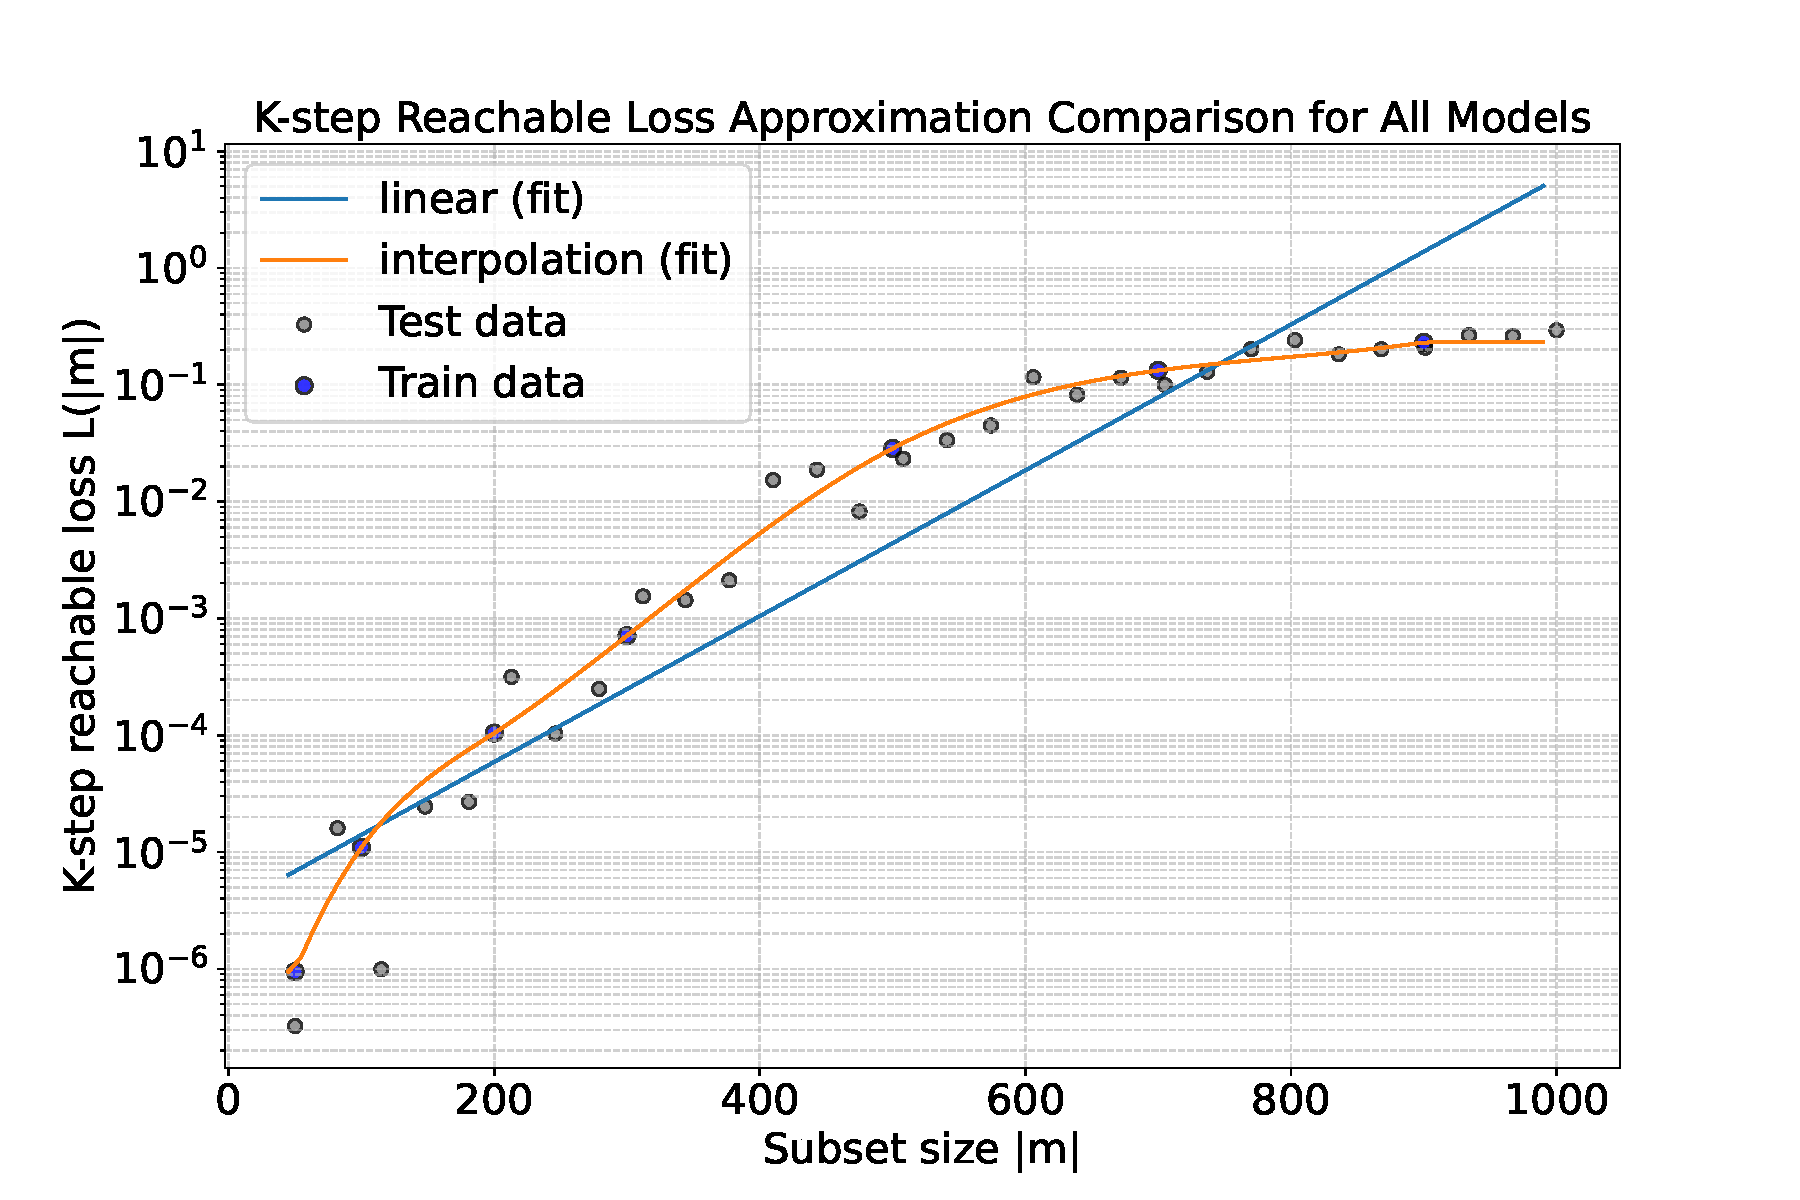
\includegraphics[width=0.8\linewidth]{pics/all_models_comparison.pdf}
  \caption{All‐models comparison of the K‐step reachable loss as a function of subset size $|m|$. Blue circles denote observed mean loss on training subsets; gray squares denote observations on held‐out test subsets. Solid curves show the fitted approximation functions for each candidate model. The vertical axis is plotted on a logarithmic scale.}
  \label{fig:appendix-fits}
\end{figure}


\subsection{Analysis of Sampling Efficiency for Loss Estimation}
\label{appendix:sampling_efficiency}

To evaluate the sample efficiency of our loss estimation method, we conducted an analysis to determine the minimum number of subset samples (\(K\)) required for reliable interpolation.

\paragraph{Experimental Design}
On the CIFAR-10 dataset with a ResNet-18 model, we evaluated the loss estimator's performance under varying sampling densities, where \(K \in \{4, 5, 6, 7, 8\}\). For each value of \(K\), we sampled \(K\) distinct subset sizes to train corresponding models, yielding \(K\) pairs of (size, loss) data points. These points were used to fit the loss estimator. Subsequently, we tested each fitted estimator on a held-out set of 100 separately sampled (size, loss) pairs to measure its interpolation accuracy.

\paragraph{Results}
The results, summarized in Table~\ref{tab:sampling_efficiency_mse}, demonstrate that the estimator's performance improves significantly up to \(K=5\) sampling points, after which the returns diminish. This indicates that our method is highly sample-efficient. Notably, increasing \(K\) further (e.g., \(K=7\)) can slightly degrade performance, likely due to overfitting the estimator to a specific set of sample points, which hinders its ability to generalize to unseen subset sizes.

\begin{table}[h]
\centering
\caption{Mean Square Error (MSE) of the loss estimator with respect to the number of sampling points (\(K\)). Performance saturates at \(K=5\), demonstrating high sample efficiency.}
\label{tab:sampling_efficiency_mse}
\begin{tabular}{cc}
\toprule
\textbf{Sampling Points (\(K\))} & \textbf{Mean Square Error} \\
\midrule
4 & 0.057668 \\
5 & 0.016326 \\
6 & 0.018594 \\
7 & 0.020031 \\
8 & 0.017905 \\
\bottomrule
\end{tabular}
\end{table}

